\chapter{Developping a DBMS Transactional Testing Framework}

\section{Overview}

This chapter presents the design, implementation and usage of a testing framework for replicating DBMS transactional bugs. Using the testing framework, we replicate a set of transactional bugs in the \textit{MySQL}, \textit{MariaDB} and \textit{TiDB} DBMSs. We then analyse the reports of the replicated bugs, and we explore the corelation between isolation levels and the reported bugs.

\section{Design}

The testing framework, is implemented in \textit{Python}, and heavily relies on \textit{Podman}, a container manager \cite{podmanwebpage} for managing DBMS instances. The tool works on \code{x64 GNU/Linux} systems, and we developped it in \textit{VSCode}, with the help of \textit{Github Copilot} \cite{copilotwebpage}.


\begin{figure}[!h]
    \centering
    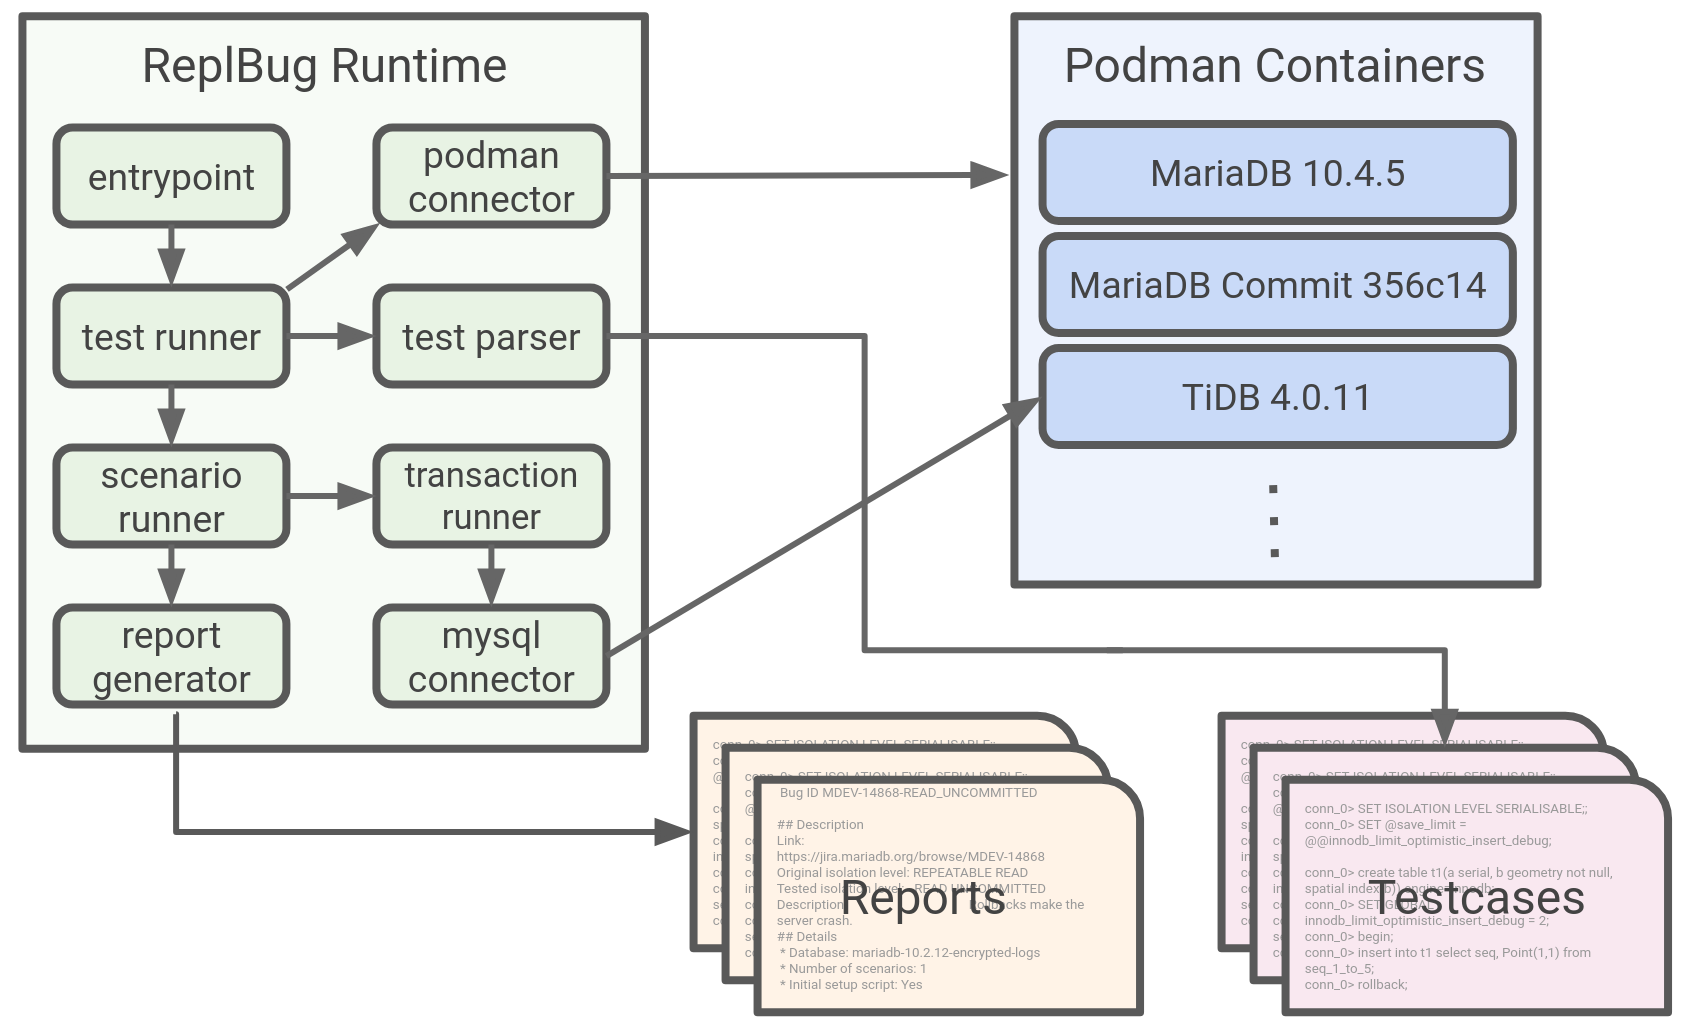
\includegraphics[width=\linewidth]{assets/replbug_design.png}
    \caption{Design of the \textit{ReplBug} testing framework}
    \label{fig:replb_design}
\end{figure}


The framework is modular, helping any future developer to easily extend it (for instance for adding support for new DBMSs). The main components in the bug testing pipeline (see Figure \ref{fig:replb_design}) are the following:

\begin{itemize}
    \item The \textit{podman connector}: This component handles the interaction with the \textit{Podman} engine, and is responsible for starting, stopping, downloading and managing containers running DBMS instances.
    \item The \textit{test parser}: This component handles the parsing of testcases, using a specific format, and is responsible for creating the internal representation of the testcases.
    \item The \textit{mysql connector}: This component handles the connection to a DBMS instance (running within a container), and is responsible for executing statements in order and extracting the results.
    \item The \textit{transaction runner}: This component handles the execution of all the statements in a transaction, and runs on different threads for concurrency.
    \item The \textit{scenario runner}: This component runs testcases under a specific configuration.
    \item The \textit{test runner}: This component orchestrates the execution of all required testcases under all specified configurations. 
\end{itemize}

\section{Custom DBMS Version}

Some bugs are specific to a certain version of a DBMS, which might not be available as pre-built binaries. For instance, versions with serious vulnerabilities are usually removed from official repositories, or intermediary versions tied to a specifig \textit{Git} commit are not released as binaries.

For the mentioned reasons, we consider the ability to built DBMSs from source essential. To simplify the process, we provide sample \textit{Dockerfile} templates, which can be used to test specific DMBS versions. A sample \textit{Dockerfile} for \textit{TiKV} can be seen in Figure \ref{fig:dockerfilesample}.
 
\begin{figure}
\begin{minted}[bgcolor=bg]{Dockerfile}
FROM golang:1.19-alpine AS builder

# Install git and other dependencies
RUN apk add --no-cache git make bash gcc wget binutils-gold \
    musl-dev curl tar

# Set the working directory inside the container and
# create necessary directories
RUN mkdir -p /go/src/github.com/pingcap
WORKDIR /go/src/github.com/pingcap

ARG TIDB_COMMIT=c9288d246c99073ff04304363dc7234d9caa5090

# Clone and build the TiDB repository
RUN git clone --depth 1 https://github.com/pingcap/tidb.git \
    && cd tidb \
    && git fetch --depth 1 origin "$TIDB_COMMIT" \
    && git checkout "$TIDB_COMMIT" \
    && make -j \
    && mv bin/tidb-server /usr/local/bin/tidb-server \
    && cd .. \
    && rm -rf tidb

EXPOSE 4000
WORKDIR /usr/local/bin
CMD ["./tidb-server", "-P", "4000"]    
\end{minted}
\caption{Sample \textit{Dockerfile} for building a specific version of \textit{TiDB}}
\label{fig:dockerfilesample}
\end{figure}

In our project, we provide \textit{Dockerfiles} for \textit{MySQL}, \textit{MariaDB} in release or debug mode, and \textit{TiDB} with or without \textit{TiKV}. Creating a new docker file only requires the \textit{Git} commit, and then running the \textit{build} command integrated into \textit{ReplBug}. 

\section{Testing Meta-Language}

For a given testcase, specifying the statements and their execution order on the DBMS is hard, due to multiple reasons:
\begin{itemize}
    \item Transactional and isolation bug PoCs usually need multiple concurent transactions, making a simple \textit{SQL} script insufficient.
    \item Some statements are expected to fail, which might lead to the termination of a standard script.
    \item The order of the statement execution (and sometimes the locking order) is important for the bug to manifest.
\end{itemize} 

To address these issues, the \textit{MySQL} development team created a testing framework which encodes testcases in a special format \cite{mysqltestrun}. Using this format, however, is cubersome, as we only need a small subset of the features, and using the \textit{MySQL} interpreter would make it hard to test other DBMSs. 

We thus create a small, custom scripting language on top of \textit{Python}, inspired by the way bug reporters describe their PoCs. In Figure \ref{fig:bug_metalanguage_sample}, we present a sample testcase for the bug \textit{MDEV-26642} in \textit{MariaDB 10.6.17}.

\begin{figure}
\begin{minted}[bgcolor=bg]{Python}
ORIGINAL_ISOLATION_LEVEL = DEFAULT_ISOLATION_LEVEL
BUG_ID = "MDEV-26642"
LINK = "https://jira.mariadb.org/browse/MDEV-26642"
DB_AND_VERSION = db_config.DatabaseTypeAndVersion(
    db_config.DatabaseType.MARIADB, "10.6.17"
)
SETUP_SQL_SCRIPT = """
create table t(a int, b int);
insert into t values (0, 0), (1, 1), (2, 2);
"""

DESCRIPTION = "The last select does not respect the update
                (a should always be 10)."


def get_scenarios(isolation_level: IsolationLevel):
    return [
        f"""
        conn_0> SET GLOBAL TRANSACTION ISOLATION LEVEL
                                {isolation_level.value};
        conn_0> begin;
        conn_0> select * from t;
        conn_1> begin;
        conn_1> update t set a = 10 where b = 1;
        conn_1> commit;
        conn_0> select * from t;
        conn_0> update t set a = 10 where true;
        conn_0> select * from t;
        conn_0> commit;
        """,
    ]
\end{minted}
\caption{Replication script for the bug \textit{MDEV-26642} in \textit{MariaDB 10.6.17}.} \label{fig:bug_metalanguage_sample}
\end{figure}

Each testcase provides the following information:
\begin{itemize}
    \item The \textit{DBMS} and version on which the bug was reported.
    \item The bug ID and a link to the bug report.
    \item The setup script, which is executed before the testcases. If the setup script is too long, it can be stored in a separate file.
    \item The description of the bug.
    \item The scenarios, which are the testcases that will be executed (one for each isolation level). Each scenario is a sequence of statements, executed in parallel by different connections.
\end{itemize}

For running a testcase, the tool provisions the required DBMS instance, executes the setup script (if present), and then runs the scenarios under all supported isolation levels. For each transaction a separate connection to the DBMS server is created. The results are then stored in a report, which can be further analysed.

\section{Usage}



\begin{figure}
    \centering
    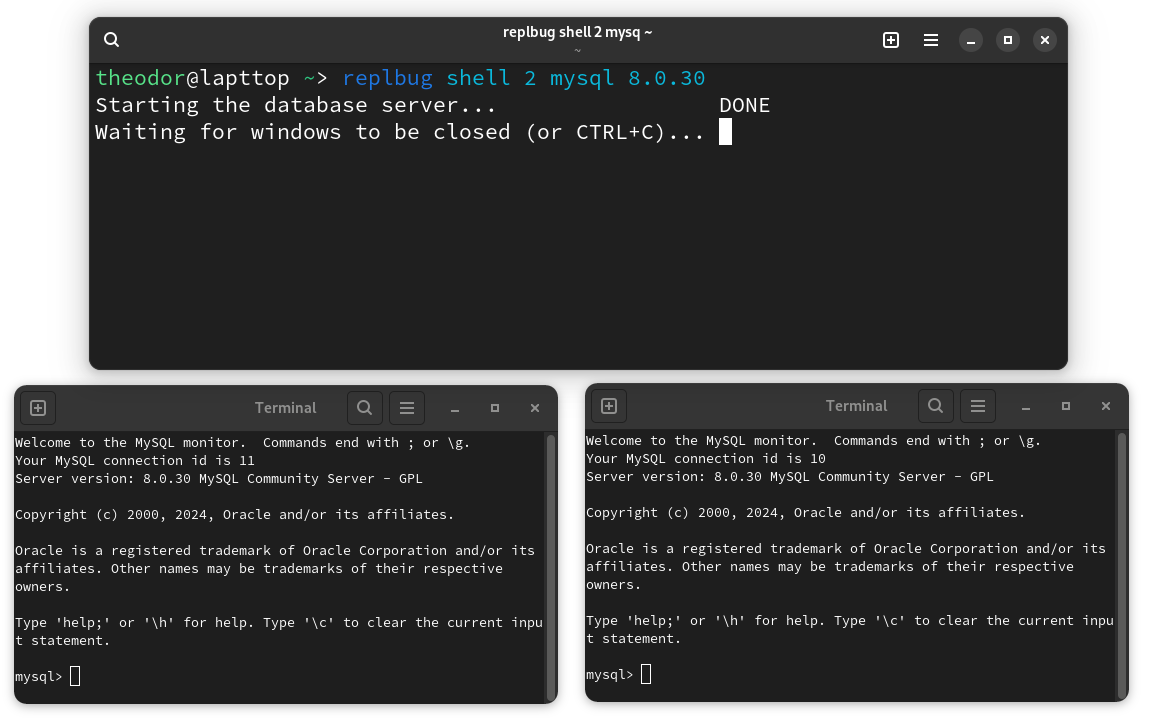
\includegraphics[width=\linewidth]{assets/replbug_shell.png}
    \caption{Using \textit{ReplBug} to start 2 \textit{MySQL v8.0.30} shells}
    \label{fig:replb_shell}
\end{figure}

\begin{figure}
    \centering
    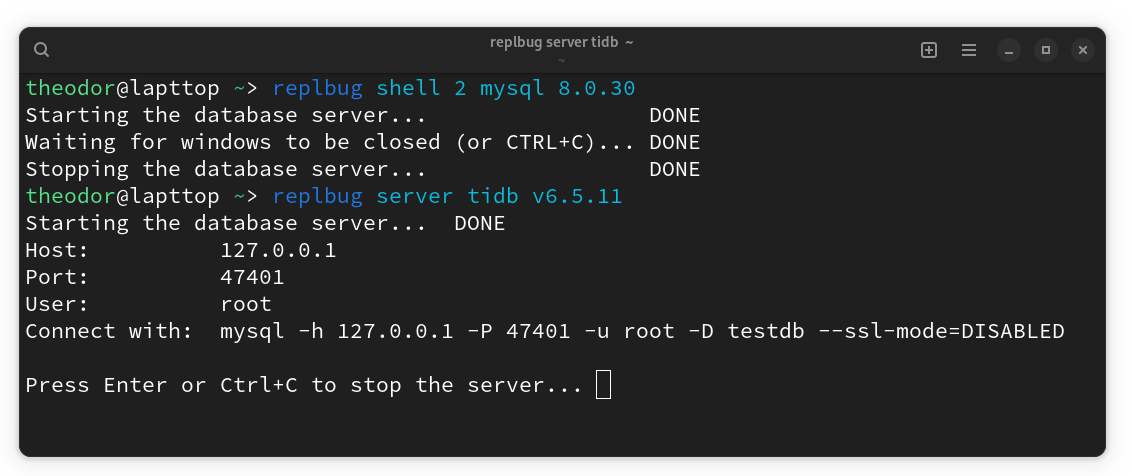
\includegraphics[width=\linewidth]{assets/replbug_server.png}
    \caption{Using \textit{ReplBug} to start a \textit{TiDB v6.5.11} server}
    \label{fig:repl_server}
\end{figure}

\begin{figure}
    \centering
    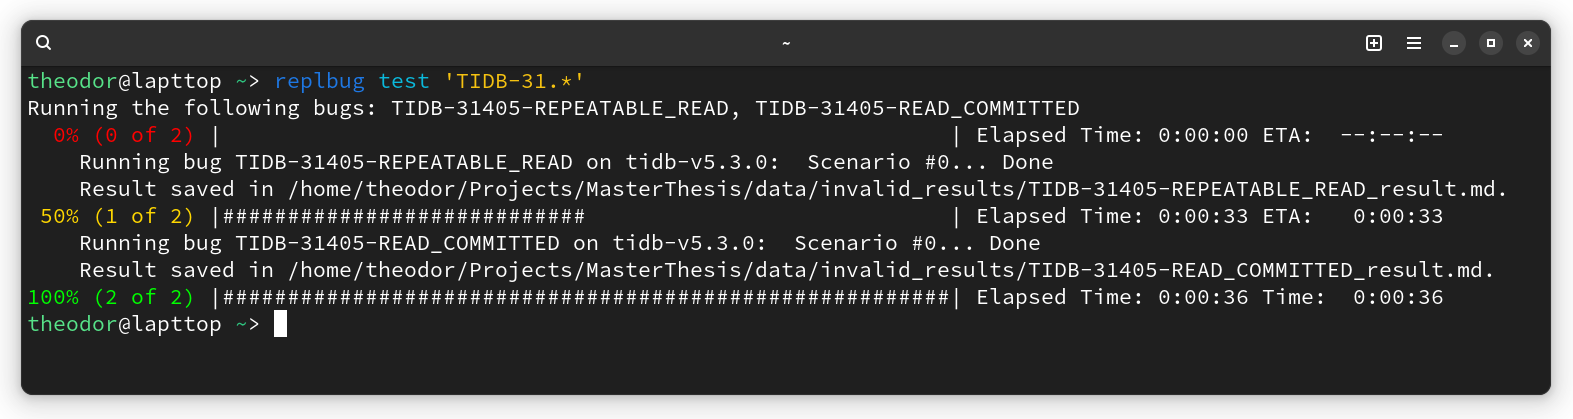
\includegraphics[width=\linewidth]{assets/replbug_test.png}
    \caption{Using \textit{ReplBug} to generate reports of some known bugs}
    \label{fig:repl_test}
\end{figure}


\begin{figure}
    \centering
    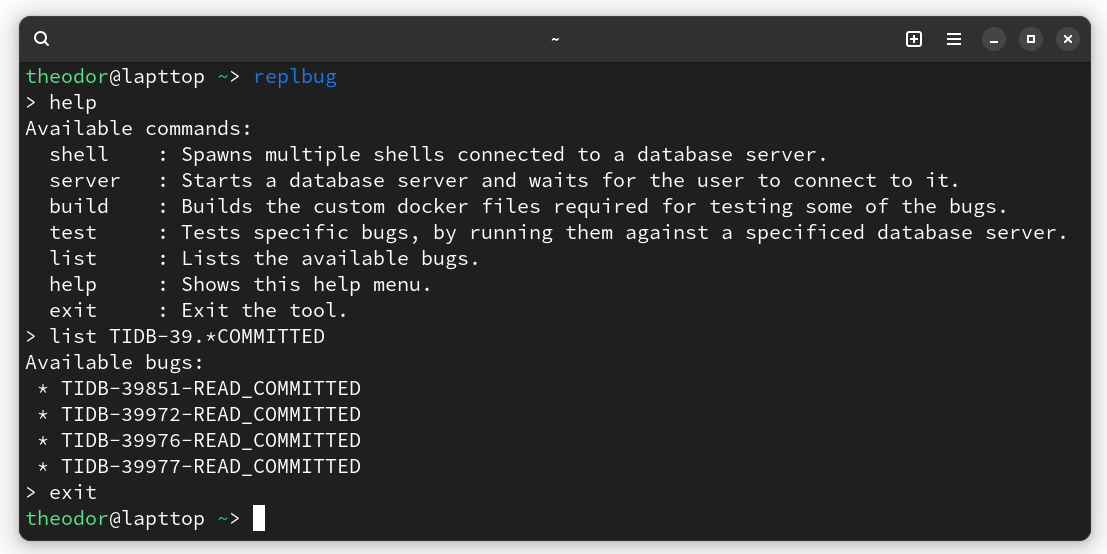
\includegraphics[width=\linewidth]{assets/replbug_interactive.png}
    \caption{Using \textit{ReplBug} in interactive mode}
    \label{fig:repl_interactive}
\end{figure}




The testing framework, called \textit{ReplBug} is invoked from the CLI. The main features it offers, exposed by the executable as subcommands are the following:
\begin{itemize}
    \item \textbf{\code{shell}} (See Figure \ref{fig:replb_shell}): Starts one or multiple \textit{MySQL}, \textit{MariaDB} or \textit{TiDB} shells, connected to a specific version of the DBMS. If the version is not present on the local machine, the tool will attempt to pull the image from Docker Hub.
    \item \textbf{\code{server}} (See Figure \ref{fig:repl_server}): Starts a specific version of the \textit{MySQL}, \textit{MariaDB} or \textit{TiDB} DBMS and provides the required details (host, port, user) for connecting to the server.
    \item \textbf{\code{test}} (See Figure \ref{fig:repl_test}): Runs the scenarios of some known bugs (which have to be written in a specific format prior), and automatically generates reports of the execution.
    \item \textbf{\code{list}}: Returns a list of the testcases available in the tool (optionally a \textit{regex} can be passed to filter the results).
\end{itemize}

The tool can be either used from the CLI by passing arguments, or in interactive mode, where the tool exposes a shell that can be used by the user  (see Figure \ref{fig:repl_interactive}).

\chapter{Replicating Transactional Bugs in MySQL, MariaDB and TiDB}

\section{Overview}

With the help of the \textit{ReplBug} testing framework, we were able to replicate \textit{MySQL}, \textit{MariaDB} and \textit{TiDB} transactional, logical and isolation bugs. We focus on transaction and isolation bugs, reported by DBMS testing papers \cite{cui2024understanding_ICSE2024, dou2023detecting_ICSE2023, cui2022differentially_ASE2022}. We then replicate the bugs on the same versions of the DBMSs, and verify which isolation levels are affected. The number of bugs taken from each paper can be seen in Figure \ref{fig:bugs_by_paper}.

\section{Replicated Bugs}


We try to replicate \textit{MySQL} and \textit{MariaDB} bugs on the $4$ isolation levels supported by the DBMSs (\textit{Read Uncommitted}, \textit{Read Committed}, \textit{Repeatable Read} and \textit{Serializable}). For \textit{TiDB}, we replicate the bugs on the $2$ isolation levels supported by the DBMS (\textit{Read Committed} and \textit{Serializable}).

\begin{figure}
    \centering
    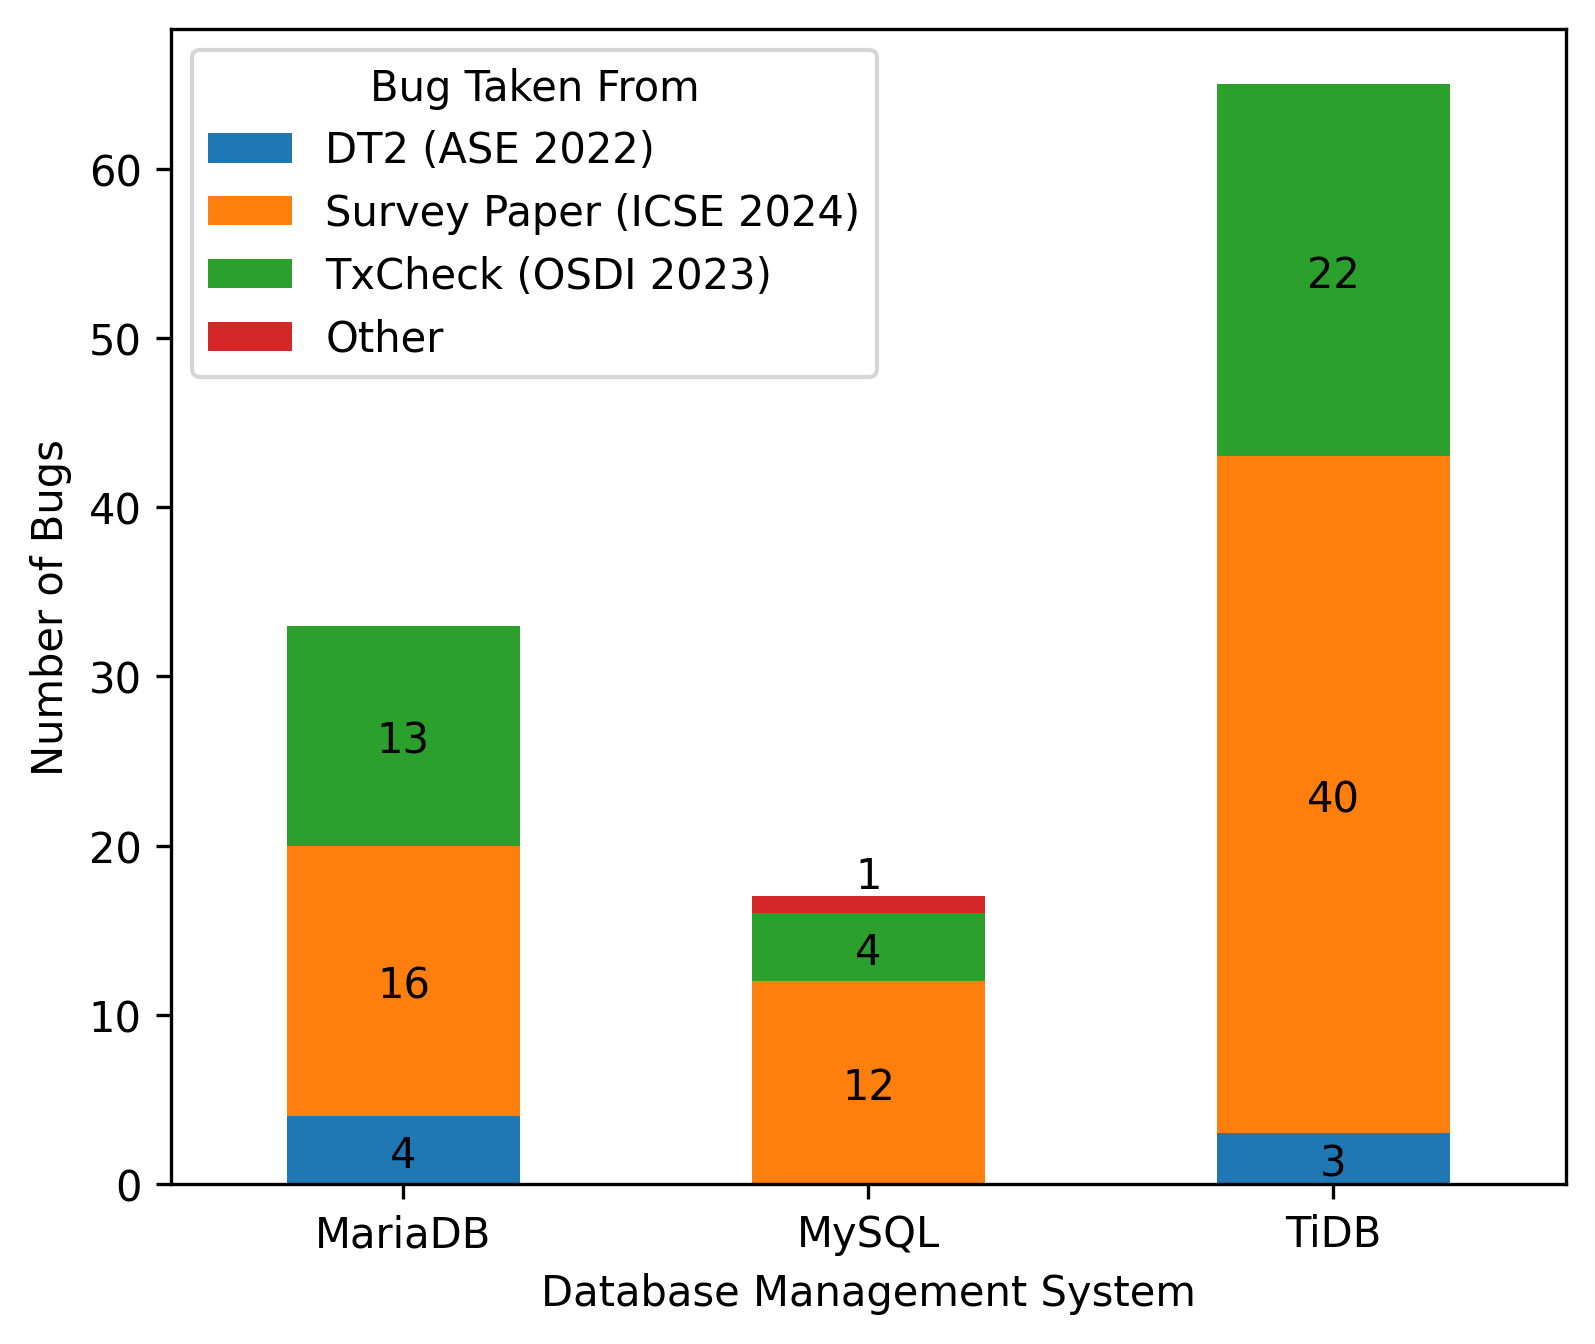
\includegraphics[width=0.8\linewidth]{assets/bug_replication_bugs_by_dbms_and_paper.png}
    \caption{Distribution of bugs by DBMS and reporting paper  \cite{cui2024understanding_ICSE2024, dou2023detecting_ICSE2023, cui2022differentially_ASE2022}.}
    \label{fig:bugs_by_paper}
\end{figure}

The methodology for replicating a bug is the following:
\begin{itemize}
    \item We search for the list of bugs reported by a paper, and filter the bugs that are transactional or isolation bugs (as reported by the paper), and manifest on one of the DBMSs we support (\textit{MySQL}, \textit{MariaDB} and \textit{TiDB}).
    \item We read the bug report in the DBMS's bug tracker, extract the version of the DBMS on which the bug was reported and a PoC.
    \item If the DBMS version is not available as a pre-built binary, we build the DBMS from source using the \textit{Dockerfile} templates provided by the \textit{ReplBug} tool.
    \item We write a testcase in the \textit{ReplBug} testing framework, using the meta-language described in the previous chapter.
    \item We run the testcase on the DBMS, under all supported isolation levels.
    \item We sometimes have to adjust the testcase, as some reports do not include the exact version of the DBMS, or the PoC is precise enough. 
\end{itemize}

Within this project, we successfully replicated $115$ bugs, out of which $33$ manifest on the \textit{MariaDB} DBMS, $17$ manifest on \textit{MySQL} and $65$ manifest on \textit{TiDB}. The distribution of the bugs by DBMS and reporting paper can be seen in Figure \ref{fig:interesting_bugs_by_paper}.

\section{Analysis}

We run the \textit{ReplBug} testing framework on the selected bugs, and we generate reports of their execution. We then read the reports, and analyse the output of the testcases. We then explore the corelation between the bugs and the isolation levels.

We find that $100$ bugs manifest on all isolation levels supported by the DBMS, and $15$ bugs only manifest on a subset of the isolation levels. In the reminder of this chapter, we refer to the bugs that manifest only on a subset of the isolation levels as \textit{interesting bugs}. In Figure \ref{fig:interesting_bugs_by_paper}, we present the distribution of the \textit{interesting bugs} by DBMS and reporting paper.

\begin{figure}
    \centering
    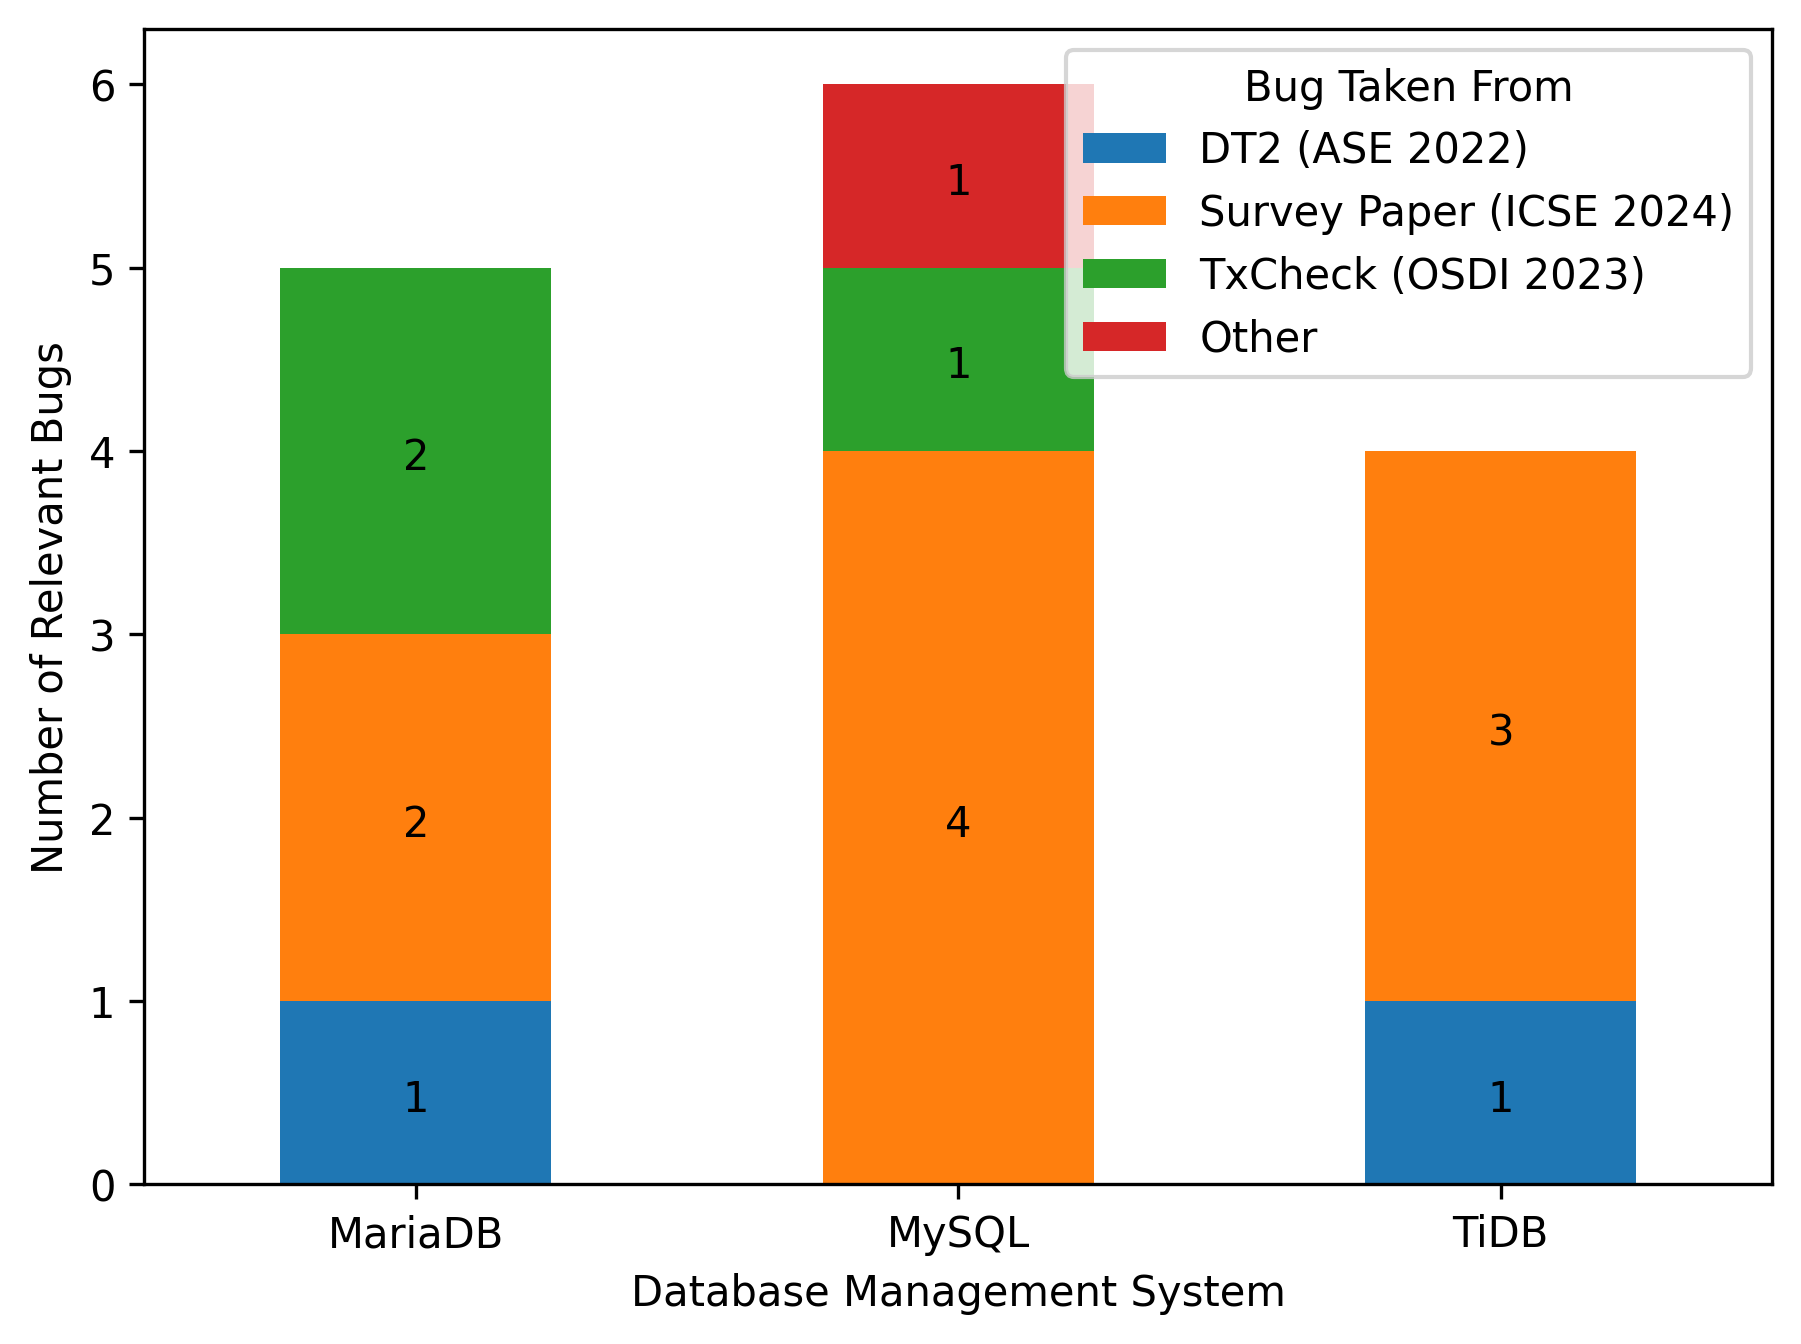
\includegraphics[width=0.8\linewidth]{assets/bug_replication_interesting_bugs_by_dbms_and_paper.png}
    \caption{Relevant bugs by DBMS and reporting paper  \cite{cui2024understanding_ICSE2024, dou2023detecting_ICSE2023, cui2022differentially_ASE2022}.}
    \label{fig:interesting_bugs_by_paper}
\end{figure}


We then explore the isolation levels under which the \textit{interesting bugs}, manifest. We find that:
\begin{itemize}
\item 5 bugs manifest under \textit{Read Committed} and \textit{Repeatable Read}.
\item 4 bugs manifest under \textit{Repeatable Read}.
\item 2 bugs manifest under \textit{Read Uncommitted} and \textit{Read Committed}.
\item 2 bugs manifest under \textit{Read Committed}.
\item One bug manifests under \textit{Serializable}.
\item One bug manifests under \textit{Repeatable Read} and \textit{Serializable}.
\end{itemize}

The findings are illustrated in Figure \ref{fig:interesting_bugs_by_isolation_lvl}. The main limitation of this analysis is that the number of \textit{intersting bugs} is small, making the results not statistically significant. Additionally, our approach only allows us to verify if a bug is triggered by a specific PoC, and not to explore the root cause of the bug, which could in theory be triggered by other PoCs under different isolation levels.

\begin{figure}
    \centering
    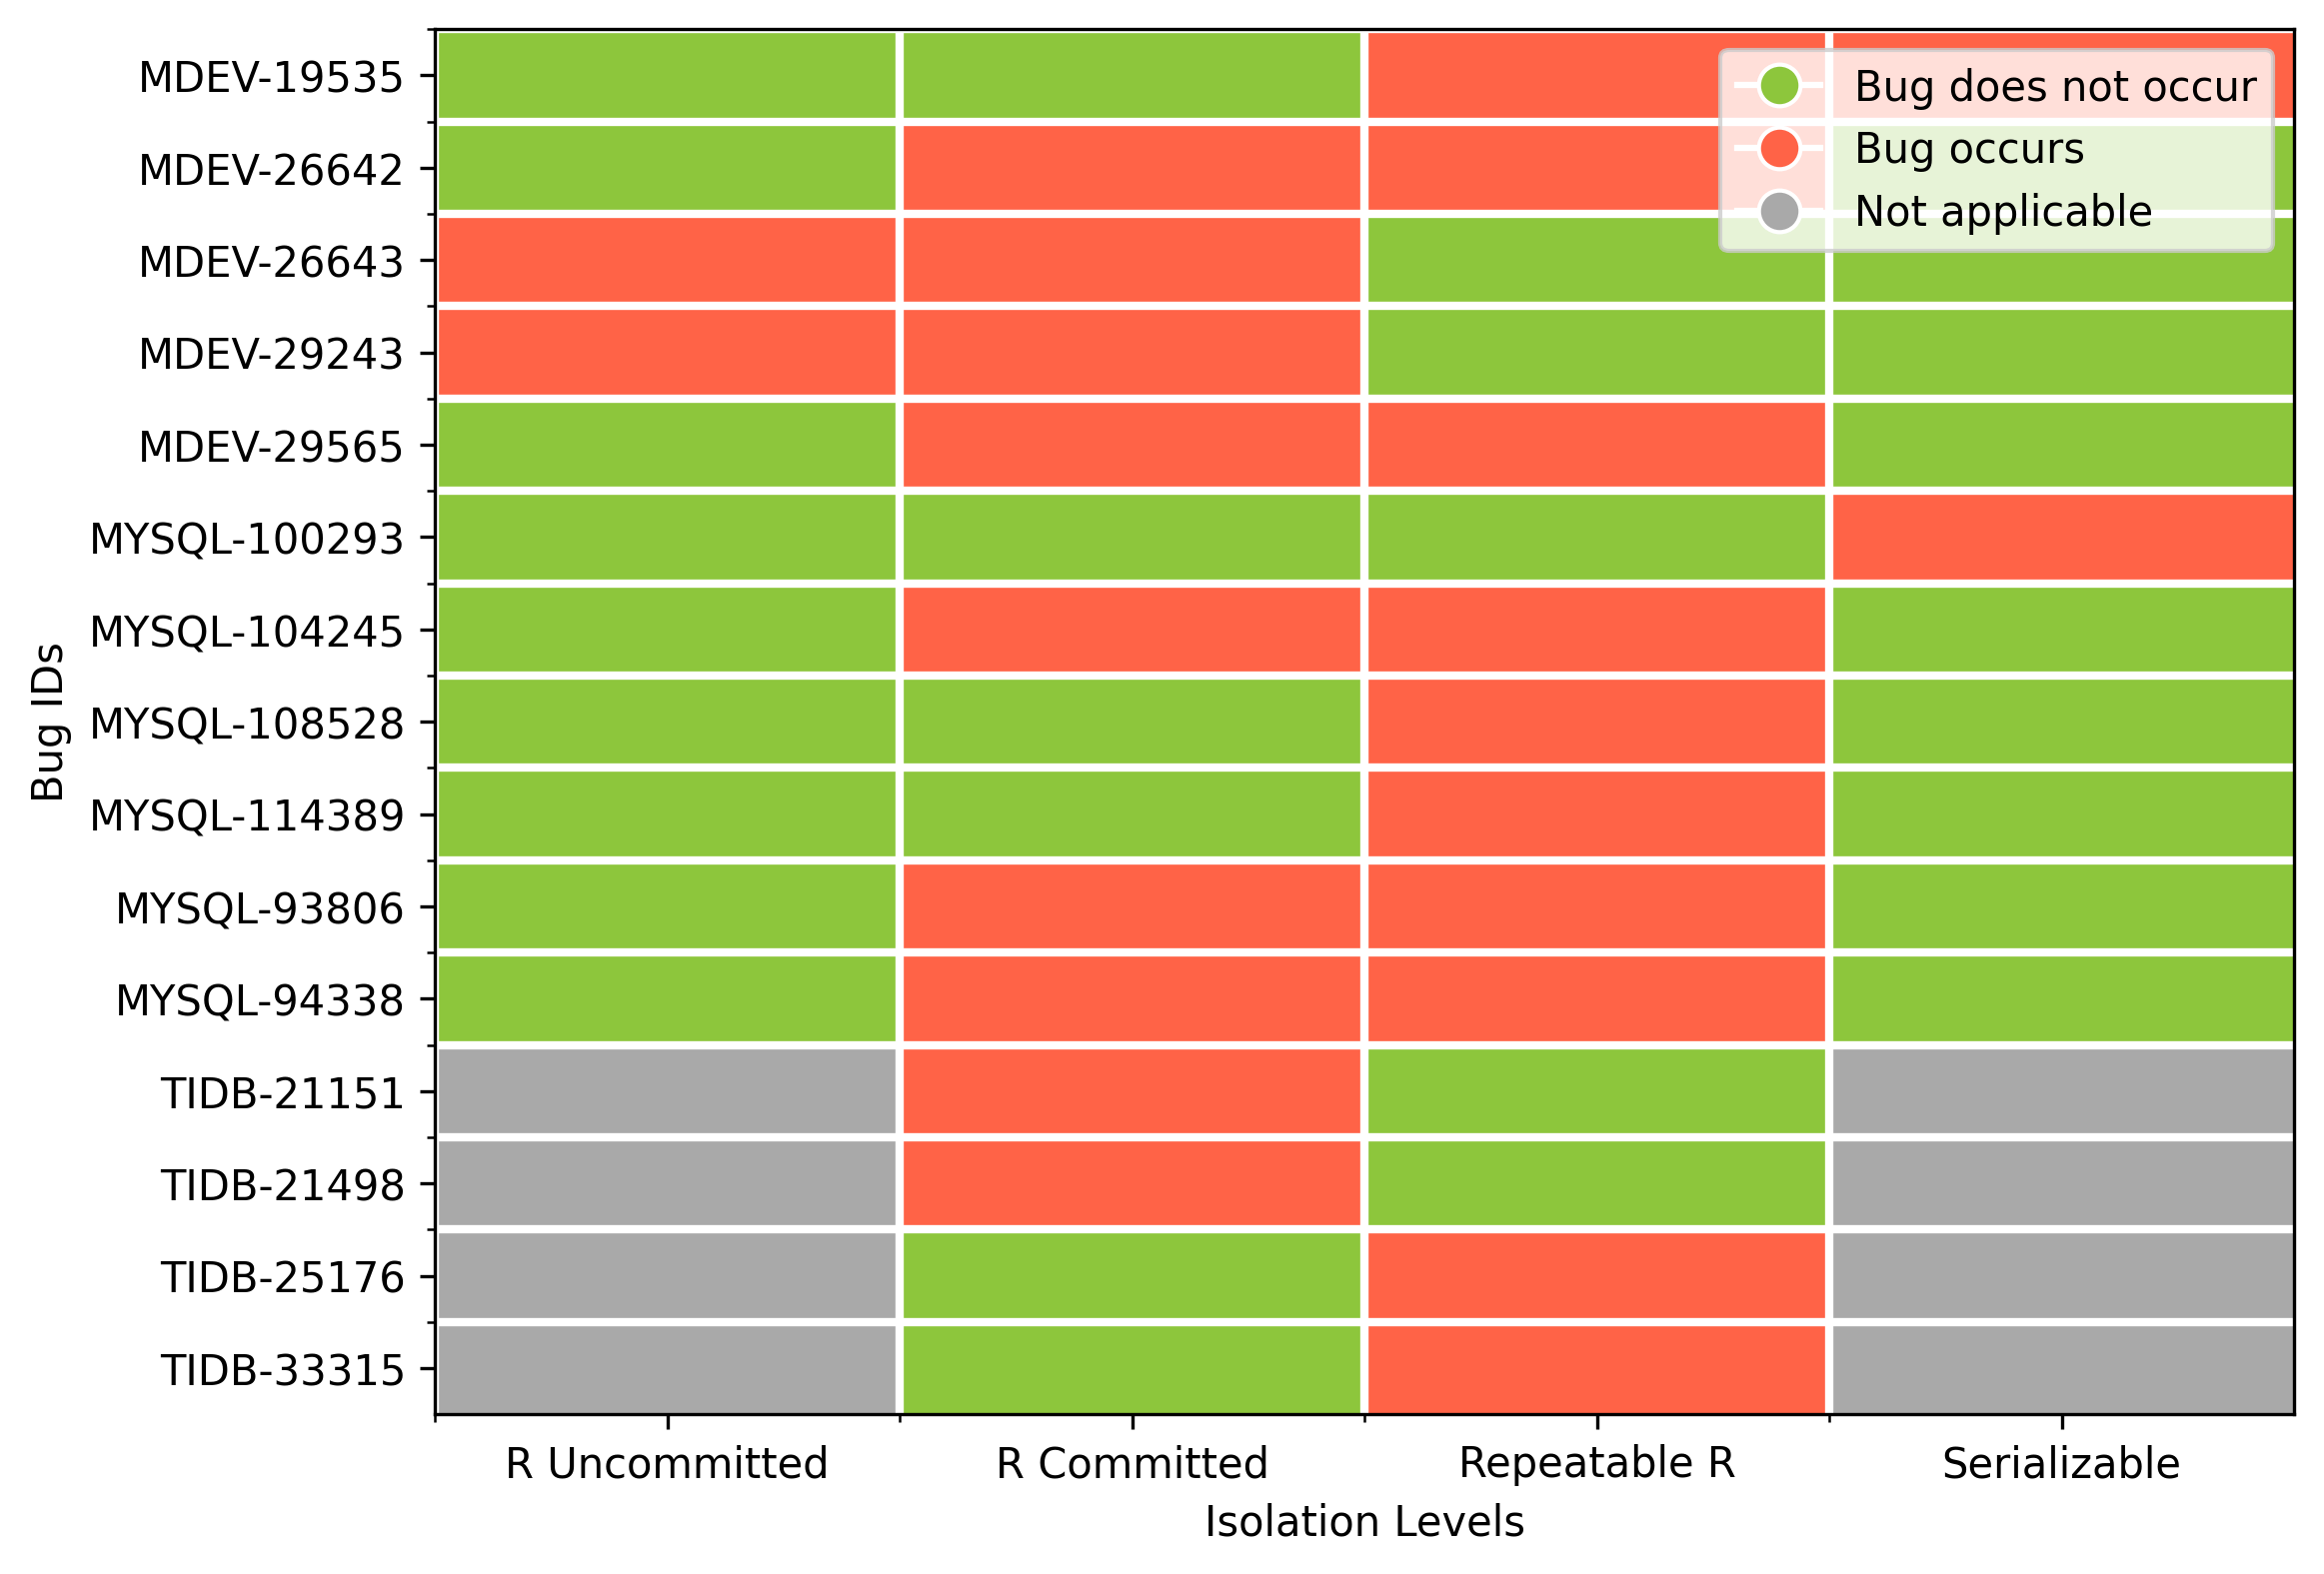
\includegraphics[width=0.9\linewidth]{assets/bug_replication_interesting_bugs_by_isolation_lvl.png}
    \caption{Relevant bugs by isolation levels.}
    \label{fig:interesting_bugs_by_isolation_lvl}
\end{figure}

\section{Interesting Bugs}

We present a brief overview of the \textit{interesting bugs}, and provide a plausible explanation for their behaviour, where possible. The bugs are presented in the order of the number of isolation levels under which they manifest.

\subsection*{Bug MDEV-19535}

This bug is replicated on \textit{MariaDB 10.4.5}, and manifests under \textit{Repeatable Read} and {Serializable}.

For compatibility, \textit{MariaDB} provides an \code{sql\_mode} variable, which can be used to mimic the behaviour of other DBMSs.

When the \code{sql\_mode} is set to \code{ORACLE}, \textit{MariaDB} ommits to add exclusive locks when running an \textit{SELECT FOR UPDATE} statement. This leads to incorrect hehaviour when running \textit{SELECT FOR UPDATE} statements under \textit{Repeatable Read} and \textit{Serializable} isolation levels, as reads are no longer guaranteed to be repeatable.

\subsection*{Bug MDEV-26642}


This bug is replicated on \textit{MariaDB 10.6.17}, and manifests under \textit{Read Committed} and \textit{Repeatable Read}. The bug was fixed by a PR in version \textit{$10.6.18$}, and was marked as affecting \textit{MySQL} too.


The bug affects concurent modifications of the same table: if a transaction updates a row of the table, and another transaction updates the entire table, the second transaction does not see its own modifications. The main part of the PoC can be seen in Figure \ref{fig:MDEV-26642}.


\begin{figure}[H]
\begin{minted}[bgcolor=bg]{SQL}
conn_0> begin;
conn_0> select * from t;        -- [(0, 0), (1, 1), (2, 2)]

conn_1> begin;
conn_1> update t set a = 10 where b = 1;
conn_1> commit;

conn_0> select * from t;        -- [(0, 0), (1, 1), (2, 2)]
conn_0> update t set a = 10 where true;
conn_0> select * from t;        -- [(10, 0), (1, 1), (10, 2)]
conn_0> commit;
\end{minted}
\caption{PoC for the bug \textit{MDEV-26642}.} \label{fig:MDEV-26642}
\end{figure}

The bug is caused by a design issue of \textit{InnoDB}, the storage engine used by both \textit{MariaDB} and \textit{MySQL}.

The bug is due to the inability of \textit{InnoDB} to detect \textit{write-write} conflicts. Under \textit{Read Committed} and \textit{Repeatable Read}, \textit{InnoDB} creates a read view at the start of a statement / transaction, used for knowing which records should be visible, but does not handle overwriten records properly. 

The \textit{Read Uncommitted} isolation level always displays the latest state of the table, and \textit{Serializable} will lock the accessed records first, so the bug does not manifest under these isolation levels.

\subsection*{Bug MDEV-26643}


This bug is replicated on \textit{MariaDB 10.5.12}, and manifests under \textit{Read Uncommitted} and \textit{Read Committed}. The bug was fixed by a PR.The PoC is very similar to \textit{MDEV-26642}, and can be seen in Figure \ref{fig:MDEV-26643}.


\begin{figure}[H]
\begin{minted}[bgcolor=bg]{SQL}
conn_0> insert into t values(null, 1), (2, 2),
                    (null, null), (null, 3), (4, null);
conn_0> begin;
conn_0> update t set a = 10 where 1;
conn_1> begin;
conn_1> update t set b = 20 where a;
conn_0> commit;
conn_1> commit;
conn_2> select * from t; 
        -- [(10, 1), (10, 20), (10, 20), (10, 20), (10, 20)]
\end{minted}
\caption{PoC for the bug \textit{MDEV-26642}.} \label{fig:MDEV-26643}
\end{figure}

The bug is caused by an improperly used semi-consistent read, where \textit{Read Uncommitted} and \textit{Read Committed} transactions are sometimes not updated with the latest changes.

\subsection*{Bug MDEV-29243}

This bug is replicated on \textit{MariaDB 10.8.3}, and manifests under \textit{Read Uncommitted} and \textit{Read Committed}, by causing a crash of the DBMS server.

The root cause of the bug is an incorrect and redundant check of the data retrival status in \textit{InnoDB}, which leads to potential assertion failures. The bug was fixed by erasing the redundant check.

\subsection*{Bug MDEV-29565}

This bug is replicated on \textit{MariaDB 10.8.3}, and manifests under \textit{Read Committed} and \textit{Repeatable Read}.

While confirmed as intented behaviour, this is caused by an poorly documented feature of \textit{InnoDB}, which allows changes made by other transactions to be visible in the current one if changes are made to the same records \cite{mysqlconsistentread}. The PoC is simplified in Figure \ref{fig:MDEV-29565}.

\begin{figure}[H]
\begin{minted}[bgcolor=bg]{SQL}
conn_1> START TRANSACTION;
conn_1> update t set a = 162;
conn_0> START TRANSACTION;
conn_1> COMMIT;
conn_0> select * from t where <CONDITION>; -- returns 1 record
conn_0> update t set a = 63 where <CONDITION>;
conn_0> select * from t where a = 63;      -- returns 2 records
conn_0> COMMIT;
\end{minted}
\caption{Simplification of the PoC for the bug \textit{MDEV-29565}.} \label{fig:MDEV-29565}
\end{figure}


\subsection*{Bug MYSQL-100293}

This bug is replicated on \textit{MySQL 5.7.31}, and manifests under \textit{Serializable}.

When the \code{innobase\_query\_caching\_of\_table\_permitted} flag is set to \code{true} (by passing \code{--query-cache-type=1} as an argument to the server), \textit{Serialisable} transactions are not blocked when using the cache, which causes some missing locks.

The bug was fixed by properly handling \code{--query-cache-type=1} when the transaction isolation level is \textit{Serializable}.

\subsection*{Bug MYSQL-104245}


This bug is replicated on \textit{MySQL 8.0.23}, and manifests under \textit{Read Committed} and \textit{Repeatable Read}.

Wen inserting rows with the same primary key multiple times (using the \code{INSERT IGNORE} statement), row locks are duplicated. Using \code{REPLACE INTO} is even worse, and adds many row locks (we believe the number of added locks is the number of matched records times the number of inserted records).

The bug only manifests on \textit{Read Committed} and \textit{Repeatable Read}, as \textit{Serializable} has a different locking mechanism, and \textit{Read Uncommitted} does not lock the records at all.

This bug dramatically increases latency, but does not cause deadlocks or crashes, as all the redundant row locks are identical. The bug is not present in \textit{MySQL 8.0} or later, so it was not fixed.

\subsection*{Bug MYSQL-108528}

This bug is replicated on \textit{MySQL 5.7.34}, and manifests under \textit{Repeatable Read}.

The bug is marked as verified, but we strongly consider the PoC actually works as intented. The PoC is simplified in Figure \ref{fig:MYSQL-108528}.

In the PoC, one transaction updates a table and commits. Another concurent transaction does not see the changes made by the first transaction, however those changes become visible when the second transaction tried to update a table. This behaviour is similar to the behaviour of \textit{MDEV-29565}, and we consider it is due to the same poorly-documented feature \cite{mysqlconsistentread}.


\begin{figure}[H]
\begin{minted}[bgcolor=bg]{SQL}
    conn_1> START TRANSACTION;
    conn_0> START TRANSACTION;
    conn_0> select * from t_rpjlsd;         -- Create snapshot.

    conn_1> update t_g6ckkb set wkey = 162; -- Update the table.
    conn_1> COMMIT;                         -- Commit.

    conn_0> select * from t_rpjlsd where
                t_rpjlsd.c_pfd8ab <= (
                    select min(wkey)
                    from t_g6ckkb
                );                          -- Affects 1 row.
    conn_0> update t_rpjlsd set wkey = 63 where
                t_rpjlsd.c_pfd8ab <= (
                    select min(wkey)
                    from t_g6ckkb
                );                          -- Affects 2 rows.
\end{minted}
\caption{Simplification of the PoC for the bug \textit{MYSQL-108528}.} \label{fig:MYSQL-108528}
\end{figure}



\subsection*{Bug MYSQL-114389}

This bug is replicated on \textit{MySQL 8.0.12}, and manifests under \textit{Repeatable Read}. The bug is still present in the latest version of \textit{MySQL} (version \textit{9.1.0}). It was closed as \textit{duplicate}, but the original bug is still open.

As the bug is still open, we do not know the root cause of the bug, whose PoC can be seen in Figure \ref{fig:MYSQL-114389}.

\begin{figure}[H]
\begin{minted}[bgcolor=bg]{SQL}
conn_0> BEGIN;

conn_1> BEGIN;                          
conn_1> UPDATE t SET b = 222, c = 333;   -- Update the table.
conn_1> COMMIT;                         

conn_2> BEGIN;
conn_2> SELECT pkId, b, c FROM t;        -- Create snapshot.

conn_0> UPDATE t SET a = 40 WHERE a = 44;
conn_0> COMMIT;

conn_2> UPDATE t SET b = 888, c = 999;   -- Update the table.
conn_2> SELECT pkId, b, c FROM t where   -- Should be empty but
          b = 854 or c = 333 order by b; -- returns a row.

\end{minted}
\caption{PoC for the bug \textit{MYSQL-114389}.} \label{fig:MYSQL-114389}
\end{figure}


\subsection*{Bug MYSQL-93806}

This bug is replicated on \textit{MySQL 8.0.12}, and manifests under \textit{Read Committed} and \textit{Repeatable Read}. The bug was fixed as part of the \textit{MySQL 8.0.16} release.

The bug is caused by a misshandling of the \code{INSERT ... ON DUPLICATE KEY} statement. When a record with a conflicting primary key is inserted, the key should be changed and a row lock created. However, under \textit{Read Committed} and \textit{Repeatable Read}, a range lock is created instead. The PoC is simplified in Figure \ref{fig:MYSQL-93806}.

\begin{figure}[H]
\begin{minted}[bgcolor=bg]{SQL}
conn_0> create table t(id int primary key, a int)engine=innodb;
conn_0> insert into t values(1,1),(5,5);

conn_0> SET GLOBAL TRANSACTION ISOLATION LEVEL REPEATBLE READ;
conn_0> begin;
conn_0> insert into t values(5,5) ON DUPLICATE
            KEY UPDATE a=a+1; -- Creates a range lock instead
                              -- of a row lock.

conn_1> begin;
conn_1> insert into t values(4, 4); -- Is needlessly blocked by
                                    -- the range lock.
\end{minted}
\caption{Simplification of the PoC for the bug \textit{MYSQL-93806}.} \label{fig:MYSQL-93806}
\end{figure}


\subsection*{Bug MYSQL-94338}

This bug is replicated on \textit{MySQL 5.7.25}, and manifests under \textit{Read Committed} and \textit{Repeatable Read}. The bug is not present in \textit{MySQL 8.0} or later, so it was not fixed.

The bug manifests by causing diry-reads when inserting multiple rows on one transaction, and performing a complex query on another transaction. The PoC is simplified in Figure \ref{fig:MYSQL-94338}. We do not know the root cause of the bug, as no bug fix was made available.

\begin{figure}[H]
\begin{minted}[bgcolor=bg]{SQL}

        conn_0> BEGIN;
        conn_1> BEGIN;

        conn_1> INSERT INTO t VALUES
                (1,40,'B',10,1),
                (1,41,'B',10,1),
                ...
                (1,40,'C',16,1),
                (1,42,'C',16,1);

        conn_0> SELECT * FROM t1
                WHERE <<CON`DITION>>; -- Dirty read.;
\end{minted}
\caption{Simplification of the PoC for the bug \textit{MYSQL-94338}.} \label{fig:MYSQL-94338}
\end{figure}

\subsection*{Bug TIDB-21151}

This bug is replicated on \textit{TiDB v4.0.8} when using the \textit{TiKV} key-value store, and manifests under \textit{Read Committed}. The bug was closed by a PR pushed to the \code{master} branch on \textit{2020-11-24}.

The bug occurs because the \code{USE\_INDEX\_MERGE} feature does not refresh the current timestamp of the transaction, causing the transaction to potentially miss the latest committed writes. While this is correct to \textit{REPETABLE READ} transactions, \textit{READ COMMITTED} transactions are expected to see committed changes. A simplified PoC can be seen in Figure \ref{fig:TIDB-21151}. 

The bug fix correctly updates the timestamp used by transactions when running under \textit{READ COMMITTED}, by invoking the \code{refreshForUpdateTSForRC} function when required.

\begin{figure}[H]
\begin{minted}[bgcolor=bg]{SQL}
conn_0> BEGIN;

-- Update the table, after transaction 0 started.
conn_1> BEGIN;
conn_1> update t set value = 11 where id = 2;
conn_1> COMMIT;

conn_0> select /*+ NO_INDEX_MERGE() */ *
            from t where a > 3 or b > 3;   -- Ok.

conn_0> select /*+ USE_INDEX_MERGE(t, ia, ib) */ *
            from t where a > 3 or b > 3;   -- Misses the update.
\end{minted}
\caption{Simplification of the PoC for the bug \textit{TIDB-21151}.} \label{fig:TIDB-21151}
\end{figure}

\subsection*{Bug TIDB-21498}

This bug is replicated on \textit{TiDB}, on the custom commit \code{3a32bd2d} using the \textit{TiKV} key-value store, and manifests under \textit{Read Committed}. The bug was closed by a PR pushed to the \code{master} branch on \textit{2021-01-12}.

The bug occurs because of missing consistency checks which allow one concurent transaction to perform DDL (Data Definition Language) operations on a table (like inserting / deleting columns or deleting indexes), while another transaction is reading from the same table. The PoC is simplified in Figure \ref{fig:TIDB-21498}.

\begin{figure}[H]
\begin{minted}[bgcolor=bg]{SQL}
conn_0> begin;

conn_1> alter table t drop index iv;
conn_1> update t set v = 11 where id = 1;

conn_0> select * from t where v = 10; -- Returns [1, 10].
conn_0> select * from t where id = 1; -- Returns [1, 11].
\end{minted}
\caption{Simplification of the PoC for the bug \textit{TIDB-21498}.} \label{fig:TIDB-21498}
\end{figure}

\subsection*{Bug TIDB-25176}

This bug was reported on a specific commit of the \code{master} branch, is replicated on \textit{TiDB 4.0.7} when using the \textit{TiKV} key-value store, and manifests under \textit{Repeatable Read}. The bug is still open as of \textit{November 2024}.

The bug is due to the usage of the \code{tidb\_snapshot} system variable, which sets the timestamp delimiting the visibility of the records \cite{tidbsnapshot}. 

Under \textit{Repetable Read}, setting this timestamp and the performing a \code{SELECT} statement breaks the isolation level guarantees. The PoC is simplified in Figure \ref{fig:TIDB-25176}.

\begin{figure}[H]
\begin{minted}[bgcolor=bg]{SQL}
conn_0> begin;                              -- Start txn.
    
conn_1> update test.ttt set a=2 where id=1; -- Update records.

conn_0> set @@tidb_snapshot=TIMESTAMP(NOW());

conn_0> select a from test.ttt where id=1;            -- [(1)].
conn_0> select a from test.ttt where id=1 for update; -- [(2)].
conn_0> select a from test.ttt where id=1;            -- [(2)].
\end{minted}
\caption{Simplification of the PoC for the bug \textit{TIDB-25176}.} \label{fig:TIDB-25176}
\end{figure}

\subsection*{Bug TIDB-33315}
